\documentclass[11pt]{article}


\usepackage{fullpage}
\usepackage{graphicx}
\usepackage{amsmath}
\usepackage{amssymb}
\usepackage{amsthm}
\usepackage{fancyvrb}

\newcommand{\myname}{Mehshan Mustafa}

\newenvironment{theorem}[2][Theorem]{\begin{trivlist}
\item[\hskip \labelsep {\bfseries #1}\hskip \labelsep {\bfseries #2.}]}{\end{trivlist}}
\newenvironment{lemma}[2][Lemma]{\begin{trivlist}
\item[\hskip \labelsep {\bfseries #1}\hskip \labelsep {\bfseries #2.}]}{\end{trivlist}}
\newenvironment{exercise}[2][Exercise]{\begin{trivlist}
\item[\hskip \labelsep {\bfseries #1}\hskip \labelsep {\bfseries #2.}]}{\end{trivlist}}
\newenvironment{problem}[2][Problem]{\begin{trivlist}
\item[\hskip \labelsep {\bfseries #1}\hskip \labelsep {\bfseries #2.}]}{\end{trivlist}}
\newenvironment{question}[2][Question]{\begin{trivlist}
\item[\hskip \labelsep {\bfseries #1}\hskip \labelsep {\bfseries #2.}]}{\end{trivlist}}
\newenvironment{corollary}[2][Corollary]{\begin{trivlist}
\item[\hskip \labelsep {\bfseries #1}\hskip \labelsep {\bfseries #2.}]}{\end{trivlist}}
\newenvironment{solution}{\begin{proof}[Solution]}{\end{proof}}
\newenvironment{idea}[2][Proof Idea.]{\textit{#1} #2}



\parindent0in
\pagestyle{plain}
\thispagestyle{plain}

\usepackage{csquotes}
\usepackage[shortlabels]{enumitem}

\newcommand{\dated}{\today}

\begin{document}

\textbf{Introduction to the Theory of
Computation}\hfill\textbf{\myname}\\[0.01in]
\textbf{Chapter 1: Regular Languages}\hfill\textbf{\dated}\\
\smallskip\hrule\bigskip

\begin{problem}{1.62}
Let $\Sigma = \{a, b\}$. For each $k \geq 1$, let $D_k$ be the language consisting of all strings that have at least one $a$ among the last $k$ symbols. Thus $D_k = \Sigma^*a(\Sigma \cup \varepsilon)^{k-1}$. Describe a DFA with at most $k + 1$ states that recognizes $D_k$ in terms of both a state diagram and a formal description.
\end{problem}

\begin{proof}
Construct the DFA $N_k = (Q,\Sigma, \delta, q_0, F)$ to recognize $D_k$:
\begin{enumerate}
\item $Q = \{q_1, q_2, \ldots, q_{k+1}\}$, where $k \geq 1$.
\item $\Sigma = \{a,b\}$.
\item $q_{0} = q_1$.
\item $F = \{q_2, \ldots, q_{k+1}\}$.
\item Define $\delta(q_i, \alpha)$ so that for any $q_i \in Q$ and any $\alpha \in \Sigma$:
\end{enumerate}

\begin{center}
$\displaystyle \delta(q_i, \alpha) \ =\begin{cases}
q_1\ & \alpha = b \text{ and } i = 1 \\
q_{i+1} & \alpha = b \text{ and } 1 < i < (k + 1) \\
q_1 & \alpha = b \text{ and } i = (k + 1) \\
q_2 & \alpha = a \\
\end{cases} \ \ $
\end{center}

\begin{center}
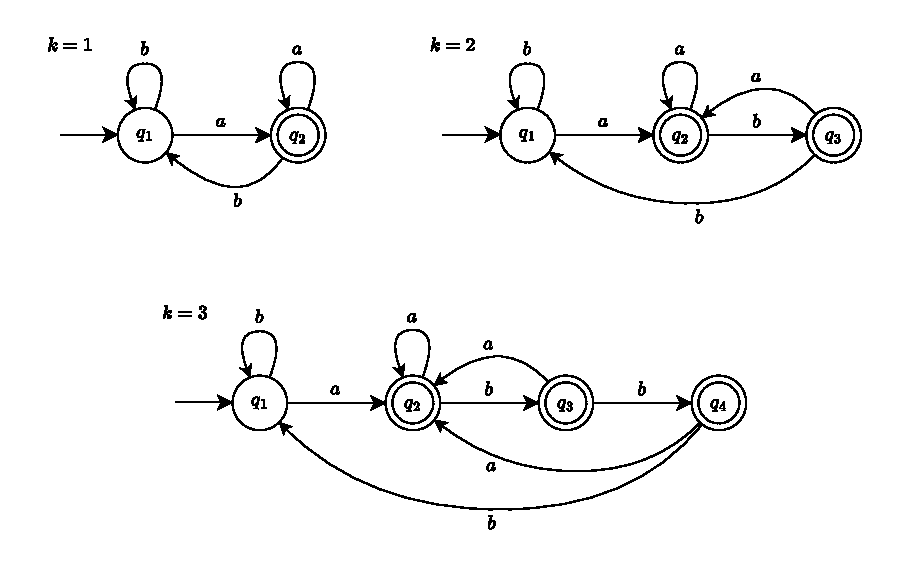
\includegraphics[scale=1.0]{Figures/Problem1.62a.pdf} \\
State diagrams of DFAs that recognize $D_{1}$, $D_{2}$ and $D_3$.
\end{center}

\end{proof}

\end{document}